\documentclass[class=article,crop=false]{standalone} \usepackage[margin=1in,headheight=57pt,headsep=0.1in]{geometry}
\usepackage[subpreambles=true]{standalone}
\usepackage{float}
\usepackage[framemethod=TikZ]{mdframed}
\usepackage{fancyhdr}
\usepackage[utf8]{inputenc} % Required for inputting international characters
\usepackage[T1]{fontenc} % Output font encoding for international characters
\usepackage{stix} % Use the STIX fonts
\usepackage{hyperref}
\hbadness=99999

\begin{document}
\subsection{Edit Tile Form}
\begin{figure}[H]
	\centering
	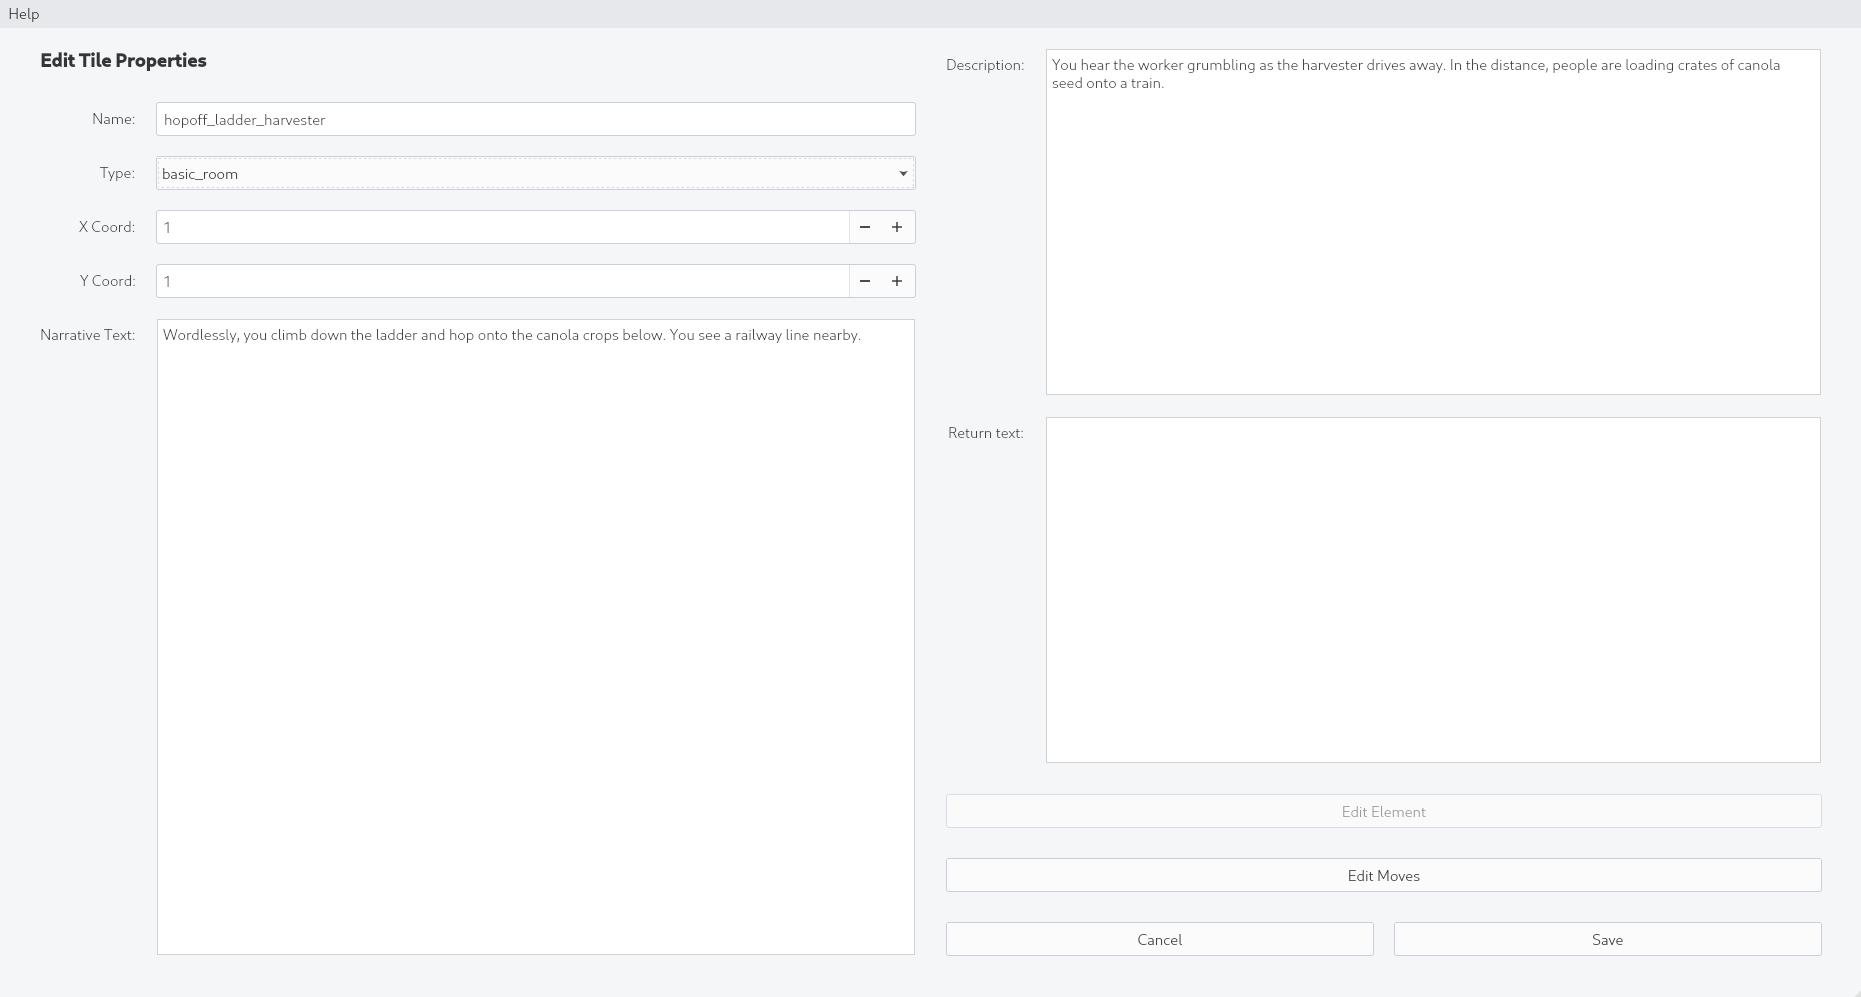
\includegraphics[width=1.0\textwidth]{./editTileFormBasic.png}
\end{figure}
Within this form you can edit the properties of individual tiles. The visible UI components for editing properties are as follows:
\begin{itemize}
	\item Name: the unique identifier for a tile, unseen by the player but cannot be reused.
	\item Type: the category of tile, which defines how the user interacts with it. Categories include \texttt{basic\_room} (simply displays text), \texttt{enemy\_room} (contains an enemy for the player to fight), \texttt{item\_room} (contains an item that the player picks up), and \texttt{victory\_room} (identical to a basic tile, except the game ends after the player enters it).
	\item X and Y Coords: the X and Y coordinate values of the tile , representing the tile's location within the game-world. Both the X and Y coordinate values must be greater than or equal to 0.
	\item Narrative Text: the words that the player sees upon entering a tile of any type for the first time.
	\item Description: the text the player sees when they enter the "\texttt{look around}" action. Should contain a more detailed description of the environment within the tile.
	\item Return Text: the text the player sees when they re-enter the tile after having visited it before. For example, if this were an \texttt{enemy\_room}, the Return Text should contain something like "a defeated enemy lies on the floor".
	\item "Edit Element": This is greyed out because the tile is currently selected to be a "\texttt{basic\_room}" type. Otherwise, this button would either open the Edit Item or Edit Enemy form, depending on whether the tile is of type "\texttt{item\_room}" or "\texttt{enemy\_room}" respectively. The text label of the button changes correspondingly as the tile type changes as well.
	\item "Edit Moves" button: this opens the Edit Moves form, allowing you to edit the list of moves for the tile.
	\item "Cancel" button: this will close the form and all sub-forms without saving any changes in the game-world..
	\item "Save" button: this will close the form and all sub-forms while saving all changes in the game-world.
\end{itemize}
\end{document}
